\documentclass[aspectratio=169]{../latex_main/tntbeamer}  % you can pass all options of the beamer class, e.g., 'handout' or 'aspectratio=43'
\usepackage{dsfont}
\usepackage{bm}
\usepackage[english]{babel}
\usepackage[T1]{fontenc}
%\usepackage[utf8]{inputenc}
\usepackage{graphicx}
\graphicspath{ {./figures/} }
\usepackage{algorithm}
\usepackage[ruled,vlined,algo2e,linesnumbered]{algorithm2e}
\usepackage{hyperref}
\usepackage{booktabs}
\usepackage{mathtools}

\usepackage{amsmath,amssymb}

\DeclareMathOperator*{\argmax}{arg\,max}
\DeclareMathOperator*{\argmin}{arg\,min}

\usepackage{amsbsy}
\newcommand{\vect}[1]{\bm{#1}}
%\newcommand{\vect}[1]{\boldsymbol{#1}}

\usepackage{pgfplots}
\pgfplotsset{compat=1.16}
\usepackage{tikz}
\usetikzlibrary{trees} 
\usetikzlibrary{shapes.geometric}
\usetikzlibrary{positioning,shapes,shadows,arrows,calc,mindmap}
\usetikzlibrary{positioning,fadings,through}
\usetikzlibrary{decorations.pathreplacing}
\usetikzlibrary{intersections}
\pgfdeclarelayer{background}
\pgfdeclarelayer{foreground}
\pgfsetlayers{background,main,foreground}
\tikzstyle{activity}=[rectangle, draw=black, rounded corners, text centered, text width=8em]
\tikzstyle{data}=[rectangle, draw=black, text centered, text width=8em]
\tikzstyle{myarrow}=[->, thick, draw=black]

% Define the layers to draw the diagram
\pgfdeclarelayer{background}
\pgfdeclarelayer{foreground}
\pgfsetlayers{background,main,foreground}

% Requires XeLaTeX or LuaLaTeX
%\usepackage{unicode-math}

\usepackage{fontspec}
%\setsansfont{Arial}
\setsansfont{RotisSansSerifStd}[ 
Path=../latex_main/fonts/,
Extension = .otf,
UprightFont = *-Regular,  % or *-Light
BoldFont = *-ExtraBold,  % or *-Bold
ItalicFont = *-Italic
]
\setmonofont{Cascadia Mono}[
Scale=0.8
]

\renewcommand{\ttdefault}{Cascadia Mono}

% scale factor adapted; mathrm font added (Benjamin Spitschan @TNT, 2021-06-01)
%\setmathfont[Scale=1.05]{Libertinus Math}
%\setmathrm[Scale=1.05]{Libertinus Math}

% other available math fonts are (not exhaustive)
% Latin Modern Math
% XITS Math
% Libertinus Math
% Asana Math
% Fira Math
% TeX Gyre Pagella Math
% TeX Gyre Bonum Math
% TeX Gyre Schola Math
% TeX Gyre Termes Math

% Literature References
\newcommand{\lit}[2]{\href{#2}{\footnotesize\color{black!60}[#1]}}

%%% Beamer Customization
%----------------------------------------------------------------------
% (Don't) Show sections in frame header. Options: 'sections', 'sections light', empty
\setbeamertemplate{headline}{empty}

% Add header logo for normal frames
\setheaderimage{
	% 
\includegraphics[height=\logoheight]{figures/TNT_darkv4.pdf}
	
\includegraphics[height=\logoheight]{../latex_main/figures/Leibniz-AI-Academy_Logo}
	% 
\includegraphics[height=\logoheight]{figures/logo_tntluh.pdf}
}

% Header logo for title page
\settitleheaderimage{
	% 
\includegraphics[height=\logoheight]{figures/TNT_darkv4.pdf}
	
\includegraphics[height=\logoheight]{../latex_main/figures/Leibniz-AI-Academy_Logo}
	% 
\includegraphics[height=\logoheight]{figures/logo_tntluh.pdf}
}

% Title page: tntdefault 
\setbeamertemplate{title page}[tntdefault]  % or luhstyle
% Add optional title image here
%\addtitlepageimagedefault{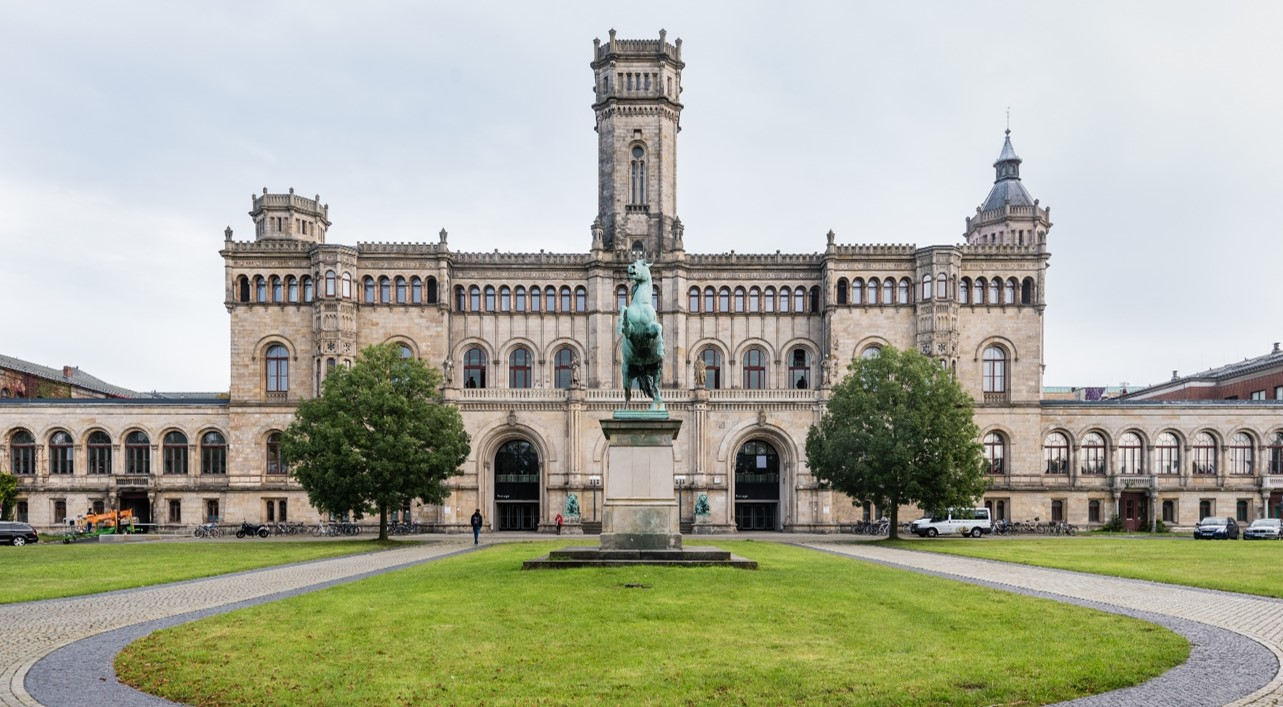
\includegraphics[width=0.65\textwidth]{figures/luh_default_presentation_title_image.jpg}}

% Title page: luhstyle
% \setbeamertemplate{title page}[luhstyle]
% % Add optional title image here
% \addtitlepageimage{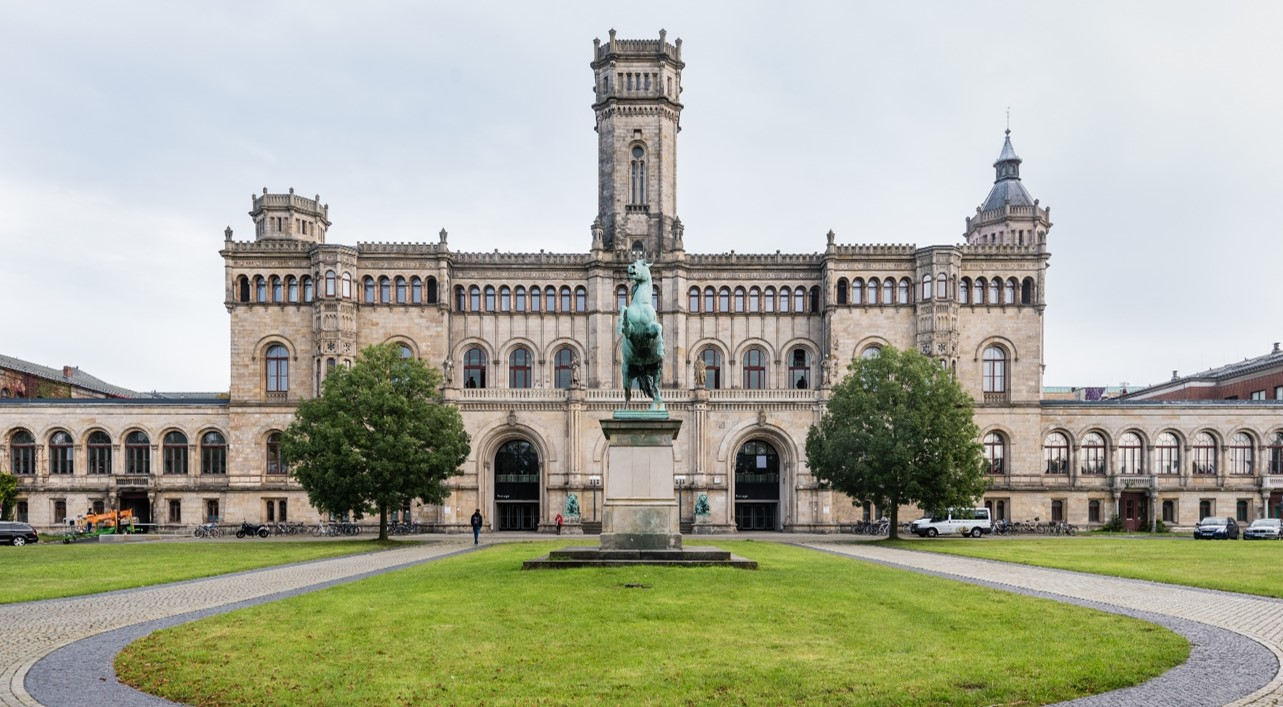
\includegraphics[width=0.75\textwidth]{figures/luh_default_presentation_title_image.jpg}}

\author[Abedjan \& Lindauer]{Ziawasch Abedjan \& \underline{Marius Lindauer}\\[1em]
	%
\includegraphics[height=\logoheight]{../latex_main/figures/luh_logo_rgb_0_80_155.pdf}\qquad
	
\includegraphics[height=\logoheight]{../latex_main/figures/DBIS_Kurzlogo.png}\qquad
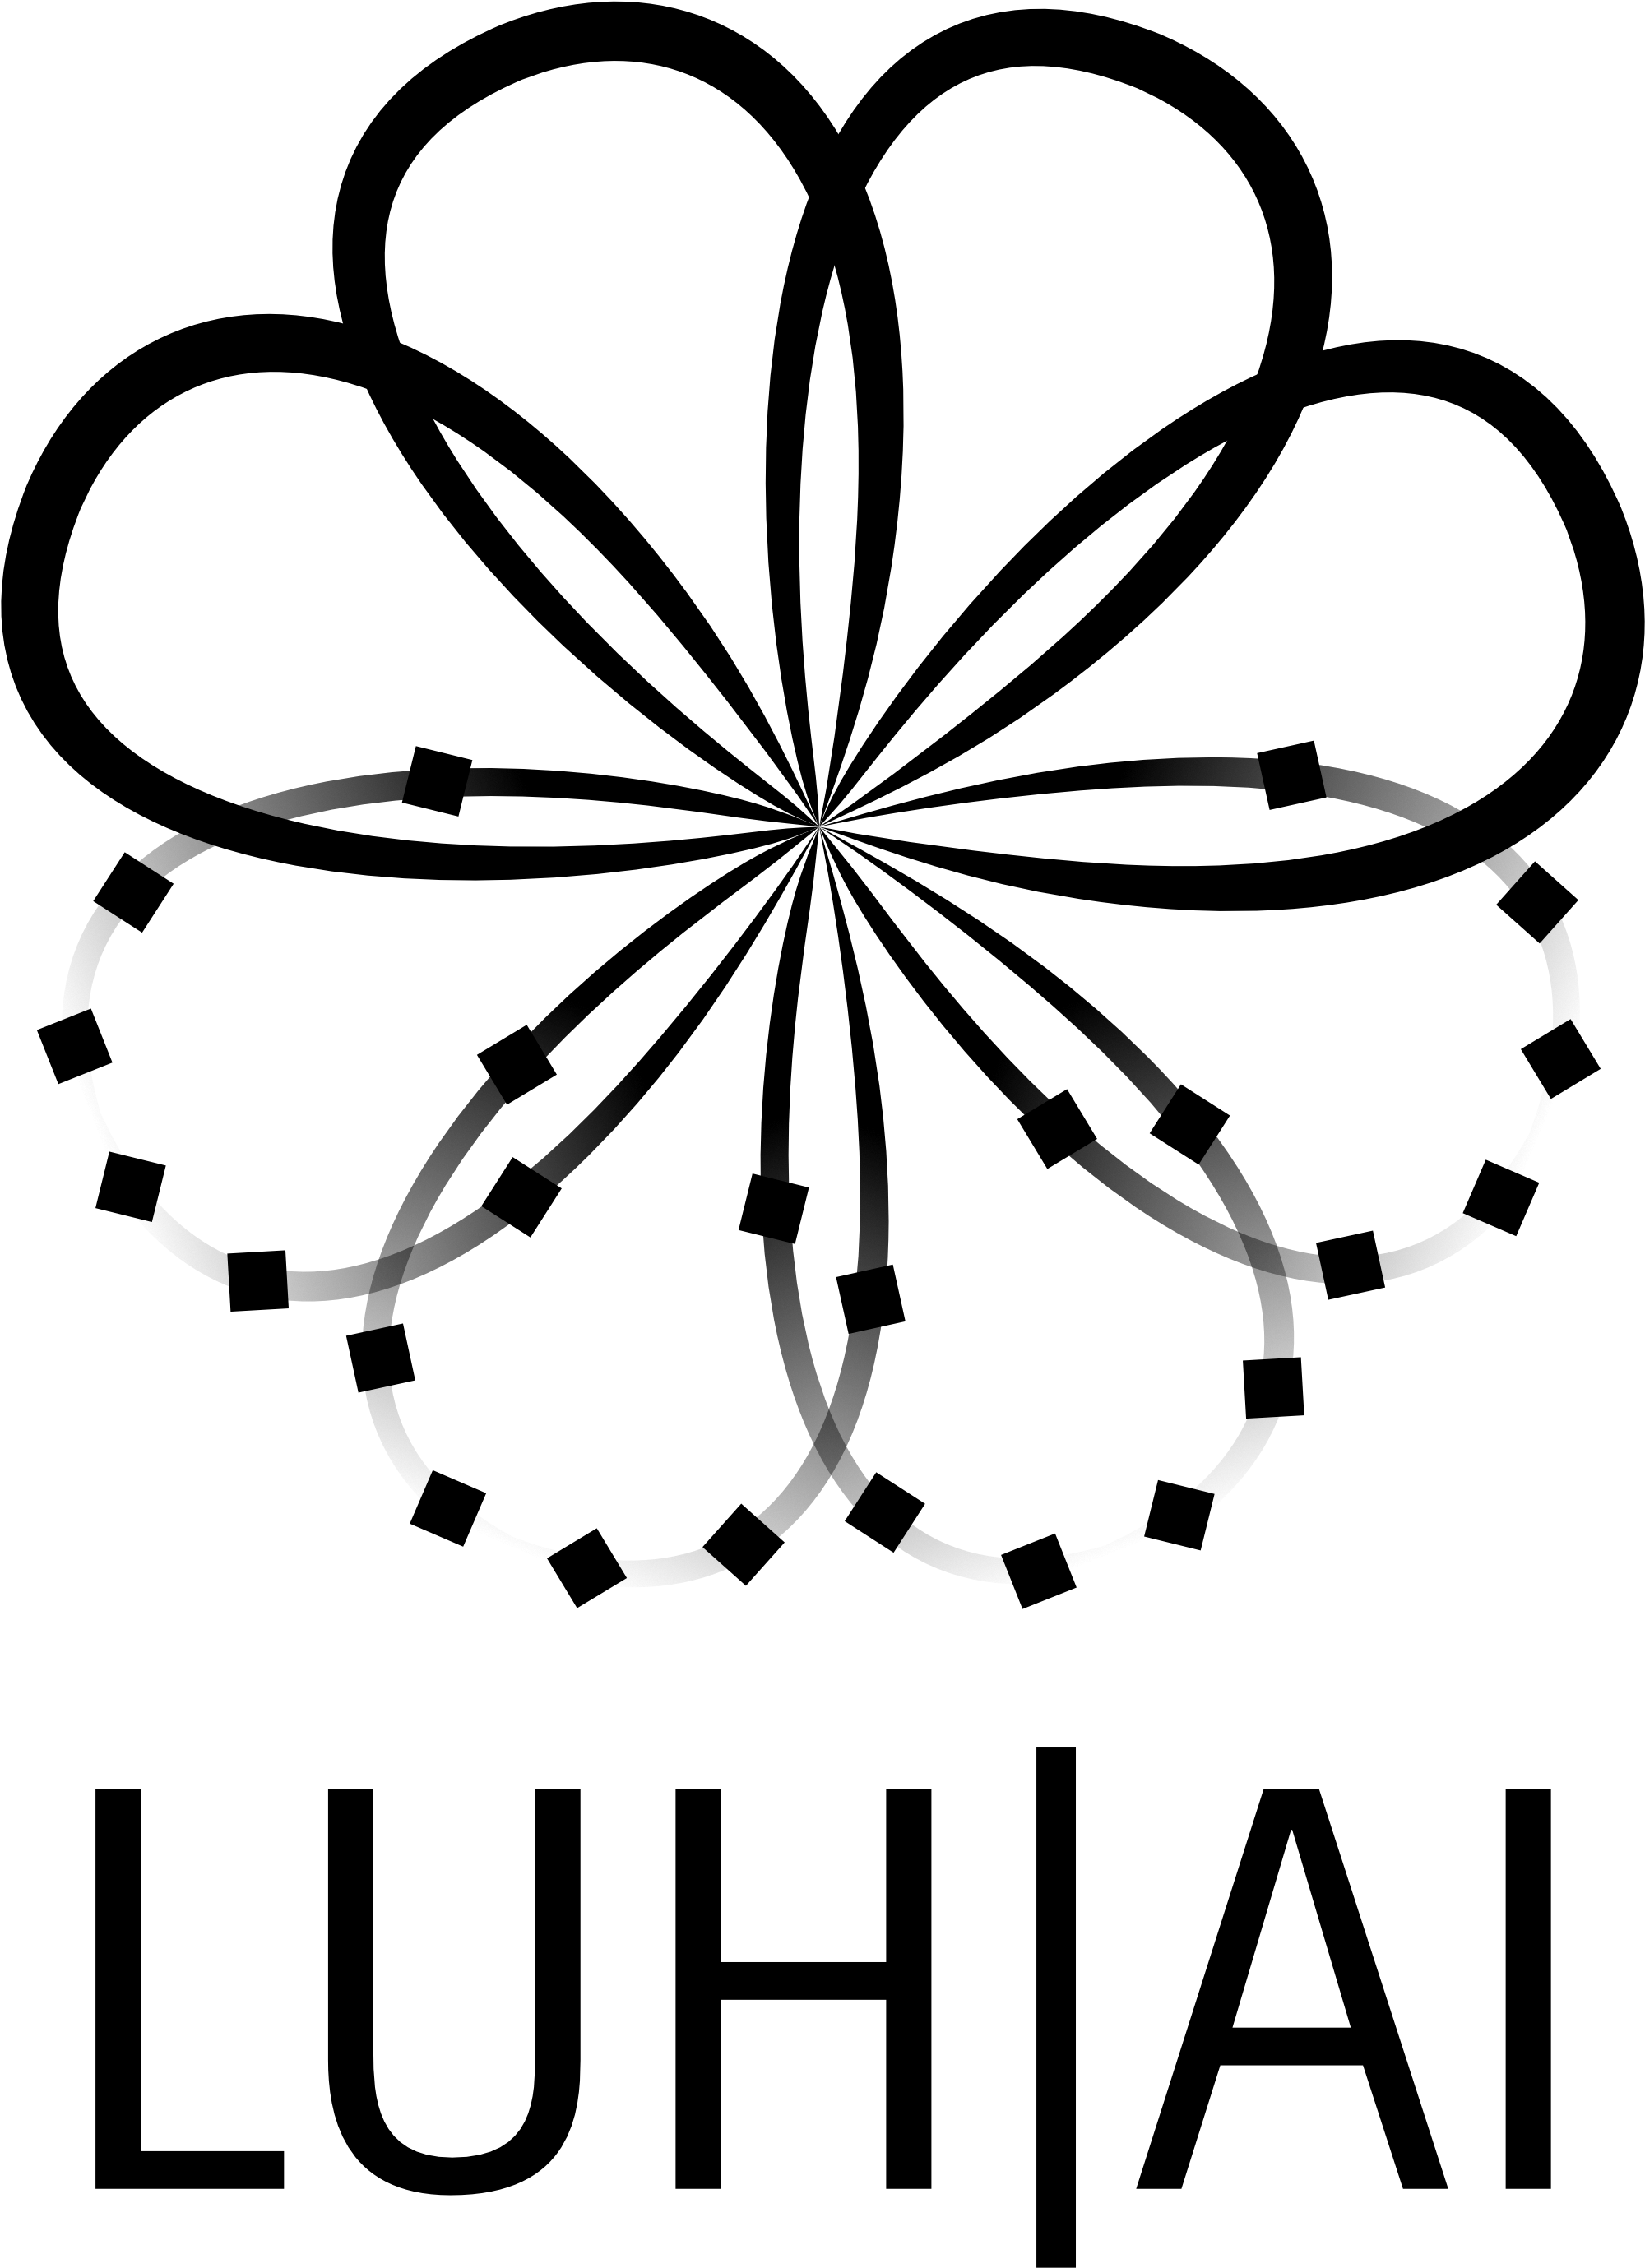
\includegraphics[height=\logoheight]{../latex_main/figures/logo_short_highres_black}\qquad

\includegraphics[height=\logoheight]{../latex_main/figures/Leibniz-AI-Academy_Logo}\qquad
%
\includegraphics[height=\logoheight]{../latex_main/figures/L3S.jpg}	
}
\date{\hspace{0.5em} {
\includegraphics[height=1.5em]{../latex_main/figures/Cc-by-nc-sa_icon.svg.png}}; extension of \href{https://ds100.org/fa21/}{[DS100]}
}


%%% Custom Packages
%----------------------------------------------------------------------
% Create dummy content
\usepackage{blindtext}

% Adds a frame with the current page layout. Just call \layout inside of a frame.
\usepackage{layout}


%%% Macros
%\renewcommand{\vec}[1]{\mathbf{#1}}
% \usepackage{bm}
%\let\vecb\bm

\title[PCA]{DS: Dimension Reduction}
\subtitle{PCA}

\graphicspath{ {./figure/} }
%\institute{}


\begin{document}
	
	\maketitle
	\begin{frame}{Dimensionality}
	    \begin{columns}
	        \begin{column}{.5\textwidth}
	               Consider the data shown. How many dimensions does this data have?
	               \begin{itemize}
	                   \item 3, because 2 weight columns are redundant
	                   \item In linear algebra terms, we’d observe that this matrix has rank 3
	                   \item More generally: Can think of a dataset’s dimensionality as the rank of the matrix representing the data 
	               \end{itemize}
	        \end{column}
	        
	        
	        \begin{column}{.5\textwidth}
	                \begin{figure}
	                    \centering
	                    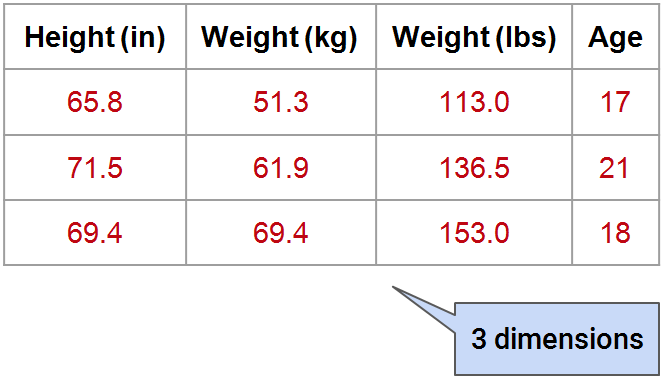
\includegraphics[scale=.4]{Bild4}
	                \end{figure}
	        \end{column}
	    \end{columns}
	\end{frame}
	
	
	\begin{frame}{Dimensionality}
	    \begin{columns}
	        \begin{column}{.5\textwidth}
	               In the previous example, we had one column that was exactly linearly dependent on another.\\
	               \bigskip
	               More generally, we want to summarize data with fewer dimensions, even if no obvious redundancies exist.
	        \end{column}
	        
	        
	        \begin{column}{.5\textwidth}
	                \begin{figure}
	                    \centering
	                    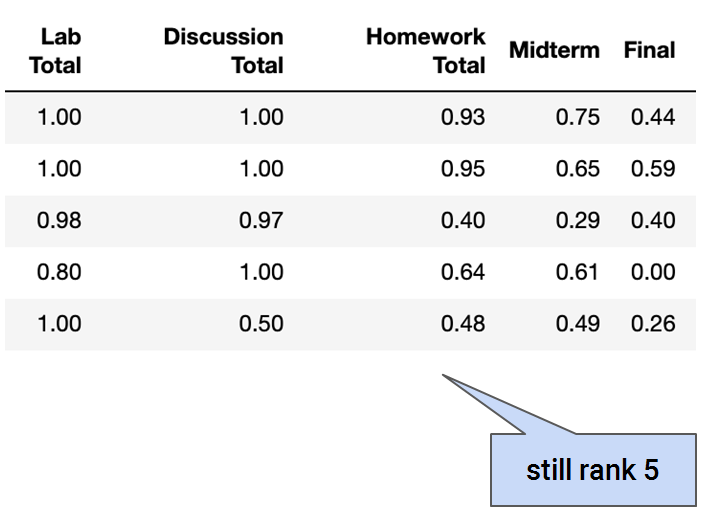
\includegraphics[scale=.4]{Bild5}
	                \end{figure}
	        \end{column}
	    \end{columns}
	\end{frame}
	
	
	\begin{frame}{Summarizing Our Data}
	    We want to summarize each student with a single “score.”
	    \begin{itemize}
	        \item We usually have a predetermined rubric (e.g. 40\% HW, 24\% Final, 10\% Discussion, etc.)
	        \item Notice the rubric is a linear combination of the features for each student.
	    \end{itemize}
	    BUT, what if we wanted a different score, one number that captures the student’s relative performance as comprehensively as possible?\\
	    \bigskip
	    We want to find a linear combination that maximizes the variance of this score.\\
	    \hfill 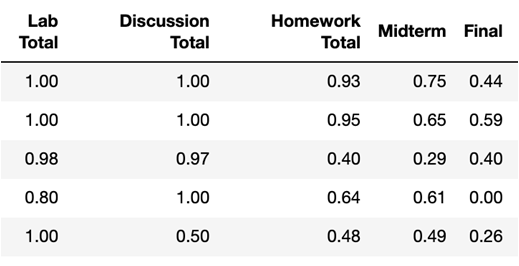
\includegraphics[scale=.6]{Bild6}
	\end{frame}
	
	
	\begin{frame}{Summarizing Our Data}
	    \begin{columns}
	        \begin{column}{.5\textwidth}
	        
	       \vspace{-2em}
	        \begin{itemize}
	            \item Let’s say we wanted to assign the “score” based only on the midterm and final exam.
	            \item Different linear combinations of the midterm and final affect the variance of our score $\rightarrow$
	            \item The variance seems to be maximized when our arrow points up and to the right (or down and to the left).
                \item \alert{Objective:} Find linear combination of features that maximizes preserved variance	           
                \begin{itemize}
                    \item Data scientists can decide dimensionality of the results space (either directly or by a threshold)
                    \item Special case of singular value decomposition (SVD)
                \end{itemize}
	        \end{itemize}
	               
	        \end{column}
	        
	        \begin{column}{.5\textwidth}
	        
	                    \centering
	                    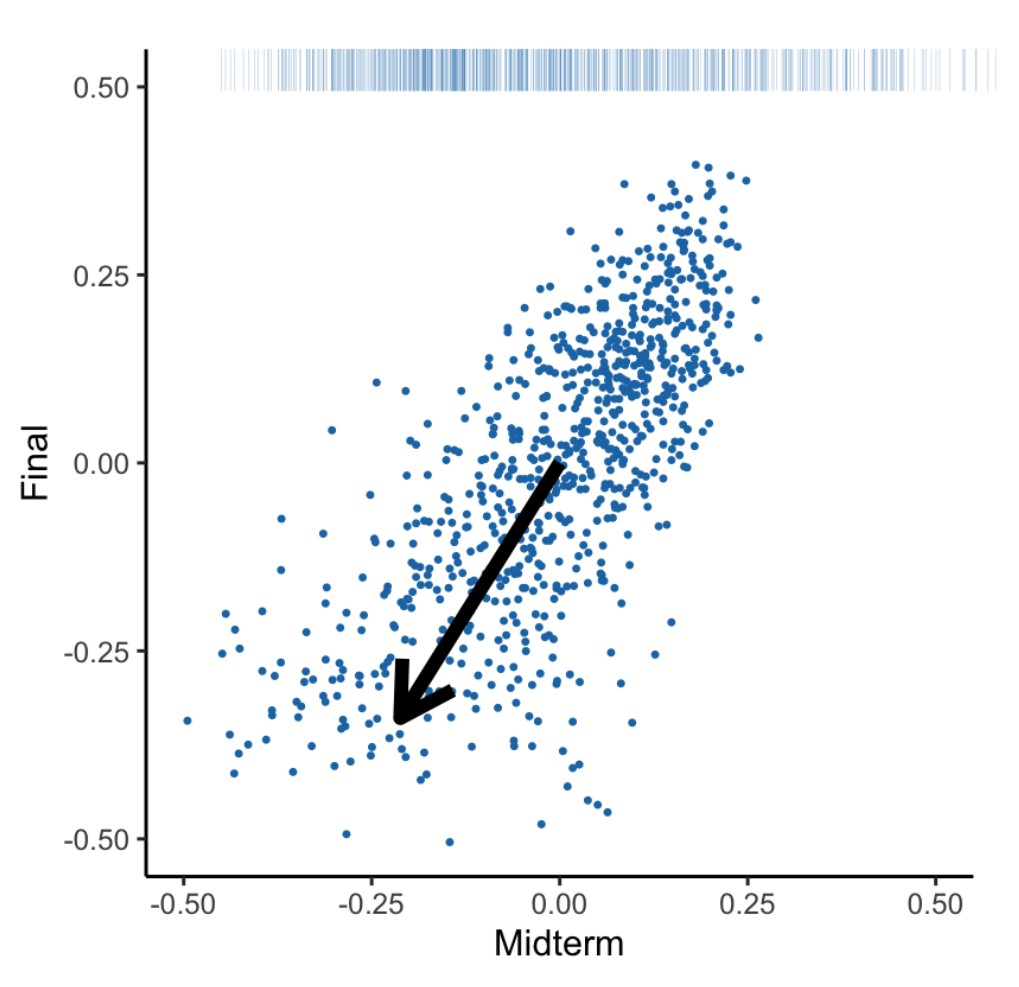
\includegraphics[scale=.1]{vect1}
	                    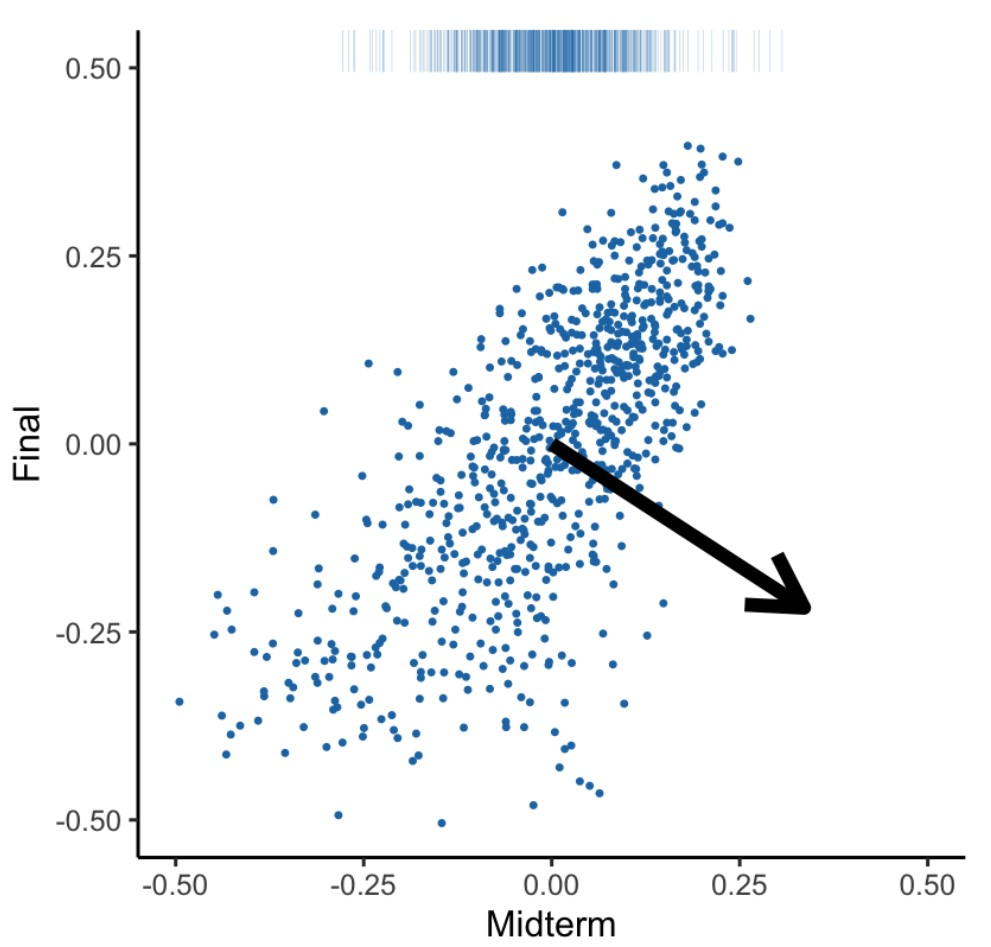
\includegraphics[scale=.1]{vect2}
	                    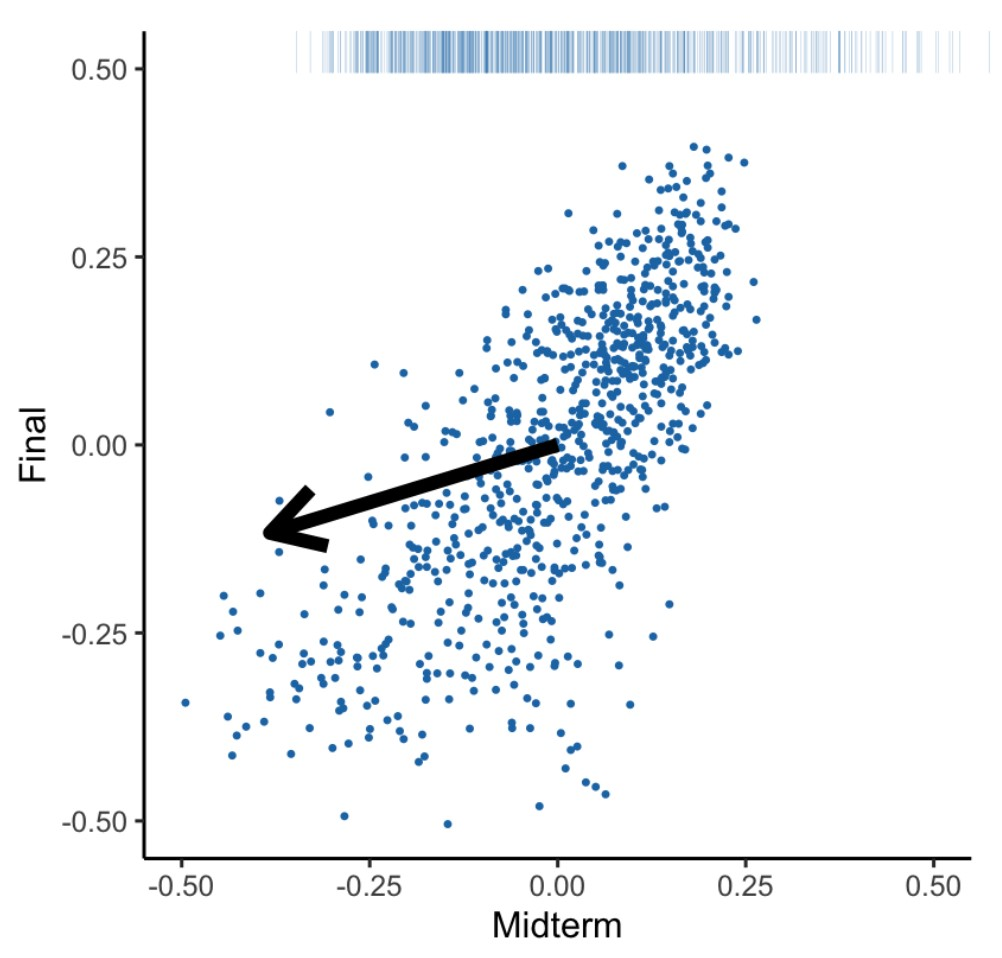
\includegraphics[scale=.1]{vect3}
	                    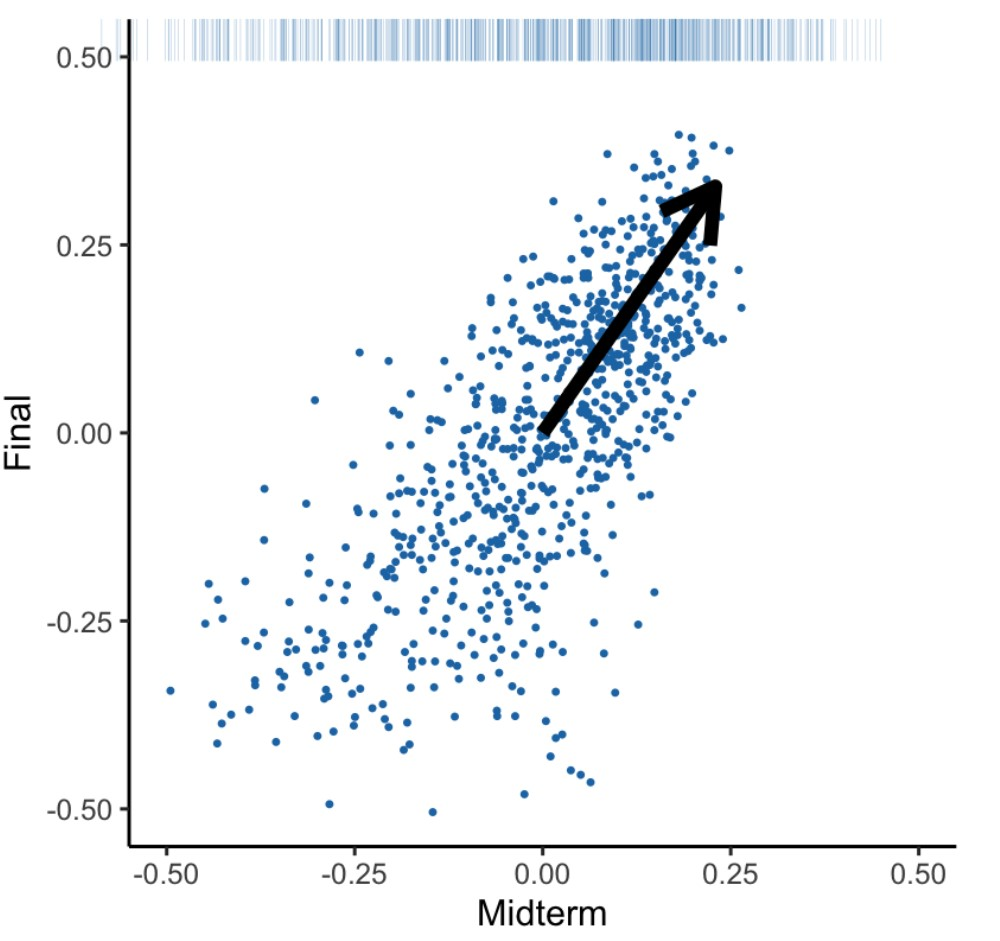
\includegraphics[scale=.1]{vect4}
	        \end{column}
	    \end{columns}
	\end{frame}
	
	\begin{frame}{Projecting Data}
        \centering
        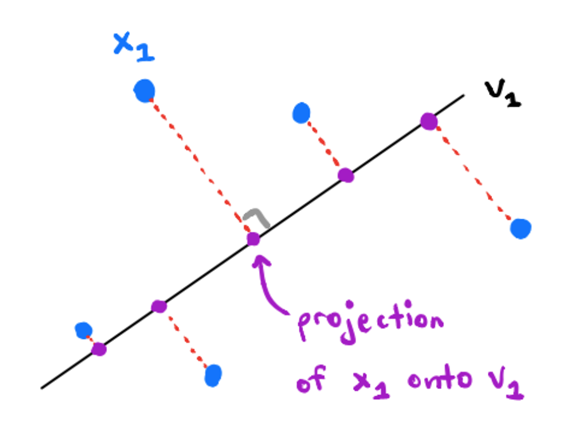
\includegraphics[width=0.5\textwidth]{Bild9.PNG}
	\end{frame}
	
	\begin{frame}{Information Quantity in each Principal Component}
        \centering
        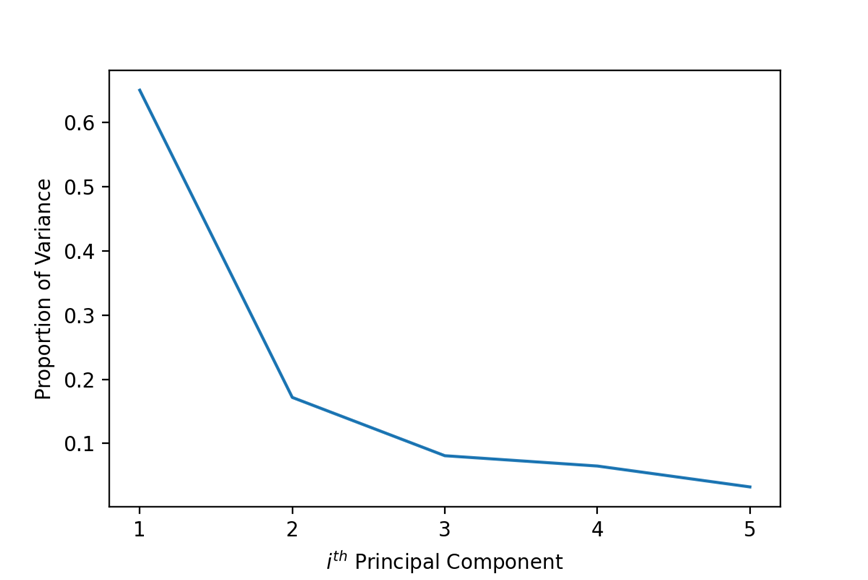
\includegraphics[width=0.5\textwidth]{Bild13.PNG}
        
        \begin{itemize}
            \item Each principal component is a vector on which your data is projected
            \item Using more will help you to preserve more of the variance in your data
        \end{itemize}
        
	\end{frame}
	
	\begin{frame}{Traits of PCA}

    Advantages:
    \begin{itemize}
        \item Can be fairly efficiently computed for medium-sized data sets
        \item Removes correlated features implicitly (because of the learned linear combination)
    \end{itemize}
    
    Disadvantages
    \begin{itemize}
        \item Assumption of linear projection --- can be circumvented with KernelPCA
        \item Defining a threshold on the proportion of variance can be hard
    \end{itemize}


	\end{frame}
	
	
\end{document}